\chapter{Was ist ein Ticket?}  % Kapitel % Steht dann über dem Text
\label{chapter:Was ist ein Ticket?}  % Steht als Text im Inhaltsverzeichnis
\index{Was ist ein Ticket?} % für das Stichwortverzeichnis

Ein Trouble Ticket lässt sich im Wesentlichen mit einem Krankenblatt eines Krankenhauspatienten vergleichen. Bei der erstmaligen Einlieferung in das Krankenhaus wird das Krankenblatt im Zuge der Anamnese neu angelegt. Jeder Arzt trägt nun seine Diagnose sowie die verordnete Therapie und Medikation ein und dokumentiert deren Erfolg. Das Krankenblatt gibt nun einen schnellen Überblick, gewährleistet eine schnelle Einarbeitung und verhindert eine Mehrfachdosierung von Medikamenten. Ist die Krankheit besiegt und der Patient entlassen, wird das Krankenblatt archiviert.\footnotemark[1]
\footnote[1]{Quelle: \href{http://otrs.org/}{http://otrs.org} }
\\
Im CodeRed System werden diese Tickets durch Betreuer, Mentoren oder Kontakte angelegt und in einer Datenbank abgelegt. Jeder der einen Patienten (Problem, Fehler) hat kann diesen in einem Ticket genau beschreiben.\\
\\
Wird ein neues Ticket erstellt wird vom System eine E-Mail Benachrichtigung an alle Mentoren des Systems versendet. Die Mentoren können sich im System das Ticket betrachten und dann eine Zuweisung an einen Betreuer oder Mentoren machen der das Ticket bearbeiten kann. \\
Alle Arbeitsschritte werden hierbei durch Workflows festgehalten. Hat der zugewiesene das Problem oder den Fehler erfolgreich behoben, so meldet er das Ticket als \qquad Fertig\qquad. Sieht der Ersteller das Problem ebenfalls als behoben so kann dieser das Ticket abschließen. Nach dem Abschließen des Ticket wird das Ticket in das Archiv verschoben.
\\
\newpage
Diese Skizzen sollen zeigen wie ein Ticket im CodeRed System läuft und wie es zugewiesen wird:\\

\begin{figure}[h]
\begin{center}
   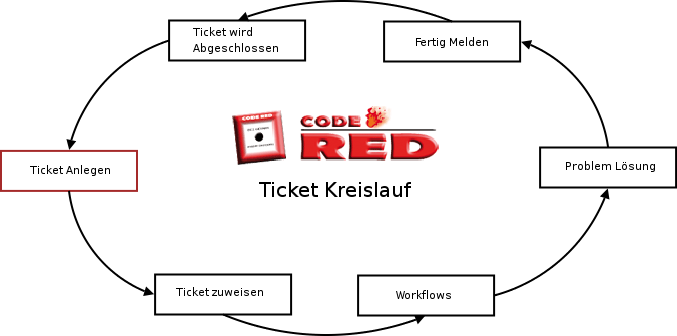
\includegraphics[width=450pt]{../bilder/Ticketkleislauf.png}
   \caption{Ticketkreislauf}
   \label{Ticketkreislauf}
\end{center}
\end{figure}
\vspace{2cm}
\begin{figure}[h]
\begin{center}
   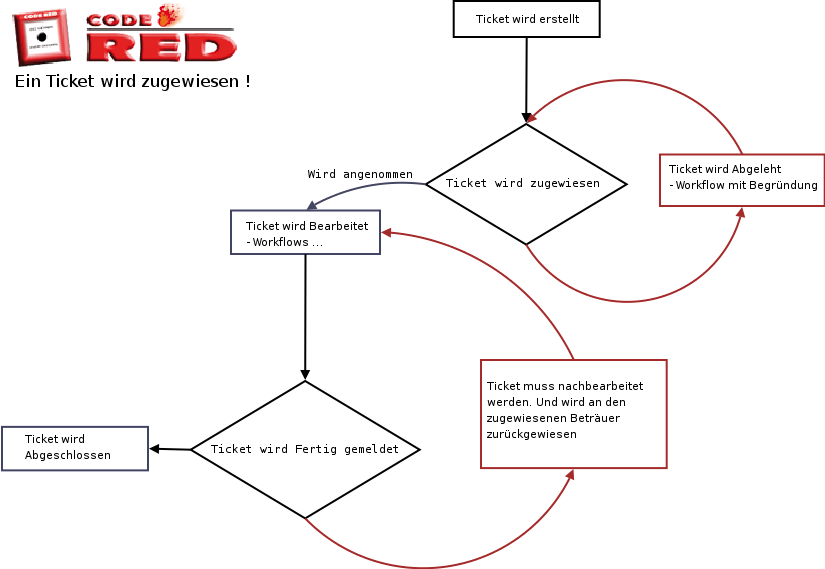
\includegraphics[width=450pt]{../bilder/Ticketzuweisung.png}
   \caption{Ticketzuweisung}
   \label{Ticketzuweisung}
\end{center}
\end{figure}

  